%==============================================================================
% Sjabloon onderzoeksvoorstel bachproef
%==============================================================================
% Gebaseerd op document class `hogent-article'
% zie <https://github.com/HoGentTIN/latex-hogent-article>

% Voor een voorstel in het Engels: voeg de documentclass-optie [english] toe.
% Let op: kan enkel na toestemming van de bachelorproefcoördinator!
\documentclass{hogent-article}

% Invoegen bibliografiebestand
\addbibresource{voorstel.bib}

% Informatie over de opleiding, het vak en soort opdracht
\studyprogramme{Professionele bachelor toegepaste informatica}
\course{Bachelorproef}
\assignmenttype{Onderzoeksvoorstel}
% Voor een voorstel in het Engels, haal de volgende 3 regels uit commentaar
% \studyprogramme{Bachelor of applied information technology}
% \course{Bachelor thesis}
% \assignmenttype{Research proposal}

\academicyear{2023-2024} % TODO: pas het academiejaar aan

% TODO: Werktitel
\title{Vul hier de voorgestelde titel van je onderzoek in}

% TODO: Studentnaam en emailadres invullen
\author{Maëlys Callens}
\email{maelys.callens@student.hogent.be}

% TODO: Medestudent
% Gaat het om een bachelorproef in samenwerking met een student in een andere
% opleiding? Geef dan de naam en emailadres hier
% \author{Yasmine Alaoui (naam opleiding)}
% \email{yasmine.alaoui@student.hogent.be}

% TODO: Geef de co-promotor op
\supervisor[Co-promotor]{N. Vermeersch (Avelon, \href{mailto:nicholas.vermeersch@avelon.be}{nicholas.vermeersch@avelon.be})}

% Binnen welke specialisatierichting uit 3TI situeert dit onderzoek zich?
% Kies uit deze lijst:
%
% - Mobile \& Enterprise development
% - AI \& Data Engineering
% - Functional \& Business Analysis
% - System \& Network Administrator
% - Mainframe Expert
% - Als het onderzoek niet past binnen een van deze domeinen specifieer je deze
%   zelf
%
\specialisation{Functional \& Business Analysis}
\keywords{Scheme, World Wide Web, $\lambda$-calculus}

\begin{document}

\begin{abstract}
  Hier schrijf je de samenvatting van je voorstel, als een doorlopende tekst van één paragraaf. Let op: dit is geen inleiding, maar een samenvattende tekst van heel je voorstel met inleiding (voorstelling, kaderen thema), probleemstelling en centrale onderzoeksvraag, onderzoeksdoelstelling (wat zie je als het concrete resultaat van je bachelorproef?), voorgestelde methodologie, verwachte resultaten en meerwaarde van dit onderzoek (wat heeft de doelgroep aan het resultaat?).
\end{abstract}

\tableofcontents

% De hoofdtekst van het voorstel zit in een apart bestand, zodat het makkelijk
% kan opgenomen worden in de bijlagen van de bachelorproef zelf.
%---------- Inleiding ---------------------------------------------------------

\section{Introductie}%
\label{sec:introductie}

Bepaalde bedrijven hebben nog steeds moeite met het ordenen van hun artikel master data. De master data gegevens worden geïdentificeerd als de kerngegevens van een organisatie. Ze bevatten gegevens over klanten, leveranciers, producten, enz. . Door het gebrek van de kwaliteit aan het bijhouden en het managen van deze gegevens hebben grote bedrijven hiee vaak moeilijkheden mee. Deze moeilijkheden kunnen vaak grote risico’s met zich meebrengen, zoals het betalen van hoge kosten om alles weer op punt te laten zetten. 

In deze bachelorproef zal er nagegaan worden hoe Machine Learning/Art Intelligence de kwaliteit van artikel master data kan verhogen. Er zal een onderzoek verricht worden naar welke technologieën er al op de markt zijn. Ook zal er nagegaan worden of het zelf maken van zo een technologie rendabel genoeg is. Op het onderzoek gebaseerd zal er een proof-of-concept opgesteld worden. 

%---------- Stand van zaken ---------------------------------------------------

\section{State-of-the-art}%
\label{sec:state-of-the-art}

% Voor literatuurverwijzingen zijn er twee belangrijke commando's:
% \autocite{KEY} => (Auteur, jaartal) Gebruik dit als de naam van de auteur
%   geen onderdeel is van de zin.
% \textcite{KEY} => Auteur (jaartal)  Gebruik dit als de auteursnaam wel een
%   functie heeft in de zin (bv. ``Uit onderzoek door Doll & Hill (1954) bleek
%   ...'')

De meeste bedrijven gebruiken tegenwoordig honderden verschillende applicaties en systemen die verschillende afdelingen doorkruisen. Bijvoorbeeld: Enterpise Resource Planning (ERP), Human Capital Management (HCM) en Customer Relationship Management (CRM). Omdat zoveel mensen de data in deze systemen aanraken, is het daardoor gemakkelijker om geïsoleerde, dubbele, verouderde of zelfs tegenstrijdige data te hebben. Slechte gegevens leiden tot slechte besluitvormingen, hierbij is het dus belangrijk om te voldoen aan de behoefte aan tijdige, accurate informatie, zelfs als de gegevensbronnen toenemen, stappen bedrijven over op master data management (MDM) \autocite{SAP}.

Master Data Management is een belangrijke methode voor het ontwikkelen en het behouden van de uniformiteit en nauwkeurigheid van de gedeelde master data van de organisatie. Met MDG kunnen bedrijven de uniformiteit en de nauwkeurigheid van hun belangrijke gegevensmiddelen verbeteren, zoals klantengegevens, productengegevens, activagegevens en locatiegegevens \autocite{Foote2023}.

Master data gegevens worden omschreven als de kerngegevens van een organisatie. Ze zijn gebaseerd op informatie die zelf veranderen en die essentieel zijn voor het runnen van de bedrijfsactiviteiten. Bedrijven verzamelen en slaan steeds meer gegevens over hun producten, gegevensmiddelen, inventaris en klanten op. Deze moeten dan beheerd blijven om accuraat te zijn. Als er onnauwkeurige master data aanwezig is in het bedrijf, is het vaak moeilijker om intelligente beslissingen over het bedrijf te maken. 

Voor de meeste bedrijvenactiviteiten zijn informatiesystemen (IS) belangrijke factoren voor de bedrijfsuitvoering en de besluitvorming. Volgens het onderzoek van \textcite{Knolmayer2006} toont aan dat ERP-systemen worden beschouwd als het centrale onderdeel van het huidige IS-landschap. Het biedt organisaties grote applicatiefunctionaliteit, die een groot deel van alle bedrijfsactiviteiten ondersteunt. Hun ontwerp belooft het probleem van gefragmenteerde informatie in grote organisaties op te lossen. Dit aan de hand van verschillende soorten gegevens uit zeer verschillende bedrijfsactiviteiten, zoals verkoop, personeelszaken, enz. samen te brengen in een consistent bedrijfsmodel. De distributie van master data wordt vaak nagegaan door een proces dat ervoor moet zorgen dat alle data wordt ingevoerd en goedgekeurd met inachtneming van de bedrijfsregels. Ook moet elke gebruiker en elk systeem nieuwe of bijgewerkte stamgegevens ontvangen zodra dat nodig is. Daardoor is het essentieel dat de kwaliteit van deze master data zo hoog mogelijk is. 

Door de technologische ontwikkelingen is men ertoe geleid dat bedrijven steeds meer data opslaan. Het onderhoud van de gegevenskwaliteit wordt echter vaak verwaarloosd daardoor kent het voor sommige bedrijven zijn dat de slechte kwaliteit van de bedrijfsgegevens hoge kosten met zich meebrengt. Het artikel van \textcite{Haug2011} toont aan dat een perfecte datakwaliteit niet vereist is, maar dat de datakwaliteit tot aan een bepaald niveau moet worden verbeterd. Het identificeren van het optimale gegevenskwaliteitsniveau is hierbij noodzakelijk.

\textcite{ Haug2011a} hebben een onderzoek uitgevoerd naar de belemmeringen voor het beheersen van de datakwaliteit in bedrijven. De eindresultaten van hun onderzoek geven aan dat een gebrek aan delegatie van verantwoordelijkheden voor het onderhouden van masterdata het enige aspect is dat de grootste impact heeft op de kwaliteit van master data. Ook blijkt dat de overgrote meerderheid van de bedrijven een standpunt heeft dat een slechte master datakwaliteit negatieve gevolgen heeft. 

%---------- Methodologie ------------------------------------------------------
\section{Methodologie}%
\label{sec:methodologie}

Voor het onderzoek naar hoe ML/AI kan gebruikt worden voor de kwaliteit van artikel master data te verhogen, is een plan van aanpak opgesteld. Dit plan van aanpak is opgesteld in verschillende fases. 

In de eerste fase is het doel om een diepgaande kennis te verwerven over het onderwerp. In de eerste deelfase zal er onderzoek gedaan worden naar relevante onderzoek artikelen, academische paper en boeken over hoe de kwaliteit van master data verhoogd kan worden. Daarna zullen de technieken en de soort gelijke oplossingen die in eerdere onderzoeken zijn vernomen onderzocht worden. 

Na de eerste fase zullen er duidelijke doelstellingen bepaald worden voor het verdere verloop van het onderzoek. In deze fase zullen de verschillende technieken en mogelijke oplossingen worden vergeleken met elkaar en zal er nagegaan worden of deze oplossingen rendabel genoeg zijn om zelf op de markt te brengen en zelf te ontwerpen. Ook zal er onderzoek verricht worden naar de specifieke concurrentie van deze mogelijkse oplossingen. 

Na deze fase zal de techniek of oplossing gekozen worden. Deze techniek of oplossing zal geselecteerd worden aan de hand van de doelstellingen die in voorgaande fases zijn vastgelegd. Als eerste zal er onderzoek gedaan worden naar welk neutraal netwerk er nodig is. Als tweede zal er moeten gezocht worden naar al dan niet bestaande libraries die we kunnen gebruiken en welke de beste is.

In de volgende fase zal er een dataset verzameld worden. Het verzamelen van een representatieve dataset is essentieel voor het succes van het onderzoek. Er zal opzoek moeten gegaan worden naar een dataset met een brede scala aan master data zodat de kwaliteit van onze oplossing kan getest worden. Om een goede dataset te vinden zal deze samengesteld worden aan de hand van datasets van specifieke bedrijven die veel gebruik maken van material master data.

In de vijfde fase zal er een proof-of-concept uitgewerkt worden. Gebaseerd op de literatuurstudie en het onderzoek zal er een proof-of-concept ontworpen worden met ML/AI, die de kwaliteit van master data mogelijks kan verhogen. De nodige middelen zullen afhankelijk zijn van welke oplossing er uit het onderzoek is gekomen. De oplossing zal getraind worden aan de hand van de verzamelde dataset. De proof-of-concept zal opgesteld worden zodanig dat als men iets wil ingeven er eerst een check gedaan wordt of deze data al dan niet al aanwezig is in de dataset zodat er geen dubbele en tegenstrijdige gegevens ingevoerd kunnen worden.

Na de uitwerking van de proof-of-concept zal er onderzoek verricht worden naar hoe deze oplossing makkelijk in de SAP master data governance (MDG) tool kan geïntegreerd worden. Er zal gekeken worden naar waar en hoe we dit best implementeren om de uitwerking ervan optimaal te kunnen benutten.

Als laatste zal er een conclusie worden getrokken uit het onderzoek en een antwoord worden geformuleerd op de onderzoeksvraag op basis van de verkregen resultaten. Er zal ook een aanbeveling geschreven worden voor de implementatie van de meest efficiënte en rendabelste techniek om de kwaliteit van artikel master data te verhogen. 

\begin{center}
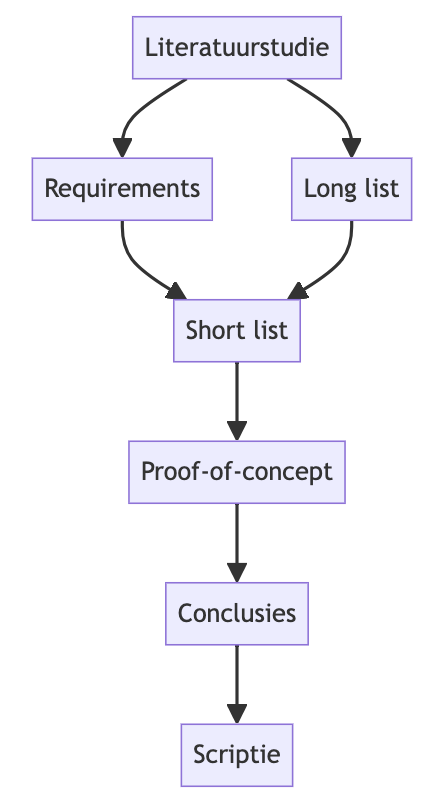
\includegraphics[scale=0.5]{methodologie.png}
\end{center}

%---------- Verwachte resultaten ----------------------------------------------
\section{Verwacht resultaat, conclusie}%
\label{sec:verwachte_resultaten}

Door te onderzoeken welke technologieën en oplossingen er al op de markt zijn in verband met master datakwaliteit kan er nagegaan worden of het al dan niet rendabel is om zelf een soortgelijke technologie op de markt te brengen. 

Het ontwikkelen van een nieuwe technologie en deze implementeren in SAP MDG Tool zal hoogstwaarschijnlijk wel rendabel zijn om zoiets op de markt te brengen. Dit is voornamelijk omdat veel bedrijven het nog steeds moeilijk hebben met het ordenen en managen van hun data. Dit is vaak doordat sommige data, zoals klantengegevens en productgegevens, door veel mensen gebruikt wordt en zo kunnen er verouderde gegevens of duplicaten ontstaan. Ook hebben nog niet veel IT-bedrijven een implementatie waarbij ML/AI de kwaliteit van artikel master data kan verhogen. Hierdoor is er nog niet veel concurrentie aanwezig op de markt, wat het ook weer veel aantrekkelijker maakt om zoiets zelf te implementeren. 

Door de proof-of-concept op te bouwen kan er veel makkelijker nagegaan worden of de data al dan niet al aanwezig is en deze desnoods moet aangepast worden. Hierdoor zouden de bedrijven veel minder duplicaten of verouderde gegevens bezitten in hun dataset en geen grote kosten meer moeten betalen om hun verwaarloosde dataset weer op punt te stellen. 



\printbibliography[heading=bibintoc]

\end{document}